\documentclass{article}
\usepackage[a4paper,margin=1in,footskip=0.25in]{geometry}
\usepackage{listings}
\usepackage{hyperref}
\hypersetup{
	 colorlinks   = true,
     citecolor    = black,
     linkcolor    = black,
     urlcolor     = black
}
\usepackage{graphicx}
\usepackage{algorithm}
\usepackage{algpseudocode}
\usepackage{amsmath}
\usepackage{tikz}
\usepackage{caption}
\usepackage{subcaption}
\usepackage{float}
\usetikzlibrary{arrows,matrix,positioning}
\setcounter{tocdepth}{3}

\begin{document}
\title{DIP Homework 2}
\author{Qiuyi Zhang 12330402 \\ \href{mailto:joyeec9h3@gmail.com}{joyeec9h3@gmail.com}} 
\date{\today}
\maketitle
\tableofcontents
\section{Exercises}

\subsection{Histogram Equalization}

\textbf{Answer:} 
Let $MN$ be the total number of pixels, $n_{r_j}$ be the number of pixels in the original image with intensity value $r_j$, $L$ be the intensity levels of the image. From eq. (3.3-8) from the textbook, the histogram equalization transformation would be:

$$s_k = \frac{(L-1)}{MN}\sum_{r_j=0}^{r_k}n_{r_j}$$

Hence $s_k$ is monotonically increasing, therefore $n_{s_k} = n_{r_k}$. The second pass of histogram equalization would produce:

$$v_k =  \frac{(L-1)}{MN}\sum_{s_j=0}^{s_k}n_{s_j}$$

Becase $n_{s_k} = n_{r_k}$, 

$$v_k =  \frac{(L-1)}{MN}\sum_{r_j=0}^{r_k}n_{r_j} = s_k$$

This shows that a second pass of histogram equalization produces exactly the same result as the first pass.

\subsection{Spatial Filtering}

\textbf{Answer:}
The merging of the bars in Fig. 1(c) is caused by the width of the filter matching the width of a bar plus the distance between the bars. When the filter is shifted between the bars, it will always cover exactly the same group of pixels that make up one bar, so the numerator for the averaging operator will always be the same within this area. Because the denominator is a constant for a given averaging filter, it will produce the same response across the area containing the bars, therefore the bars seem to be merged. But in Fig. 1(b) and Fig. 1(d), the width of the filter is smaller/larger than, or not a multiple of, the width of a bar plus the distance between the bars. Therefore there are no merging effects in these two figures.

% -------------------- Programming Tasks ------------------------
\section{Programming Tasks}
% -------------------- Histogram Equalization ------------------------
\subsection{Histogram Equalization}
% -------------------- Results ------------------------
\subsubsection{Results}
\begin{figure}[H]
	\centering
	% pt = px * 72 / DPI
	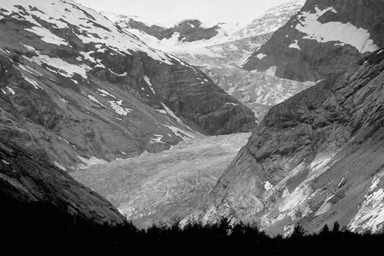
\includegraphics[width=288pt]{../img/02.png}
	\caption{The original image}
\end{figure}

\begin{figure}[H]
	\centering
	% pt = px * 72 / DPI
	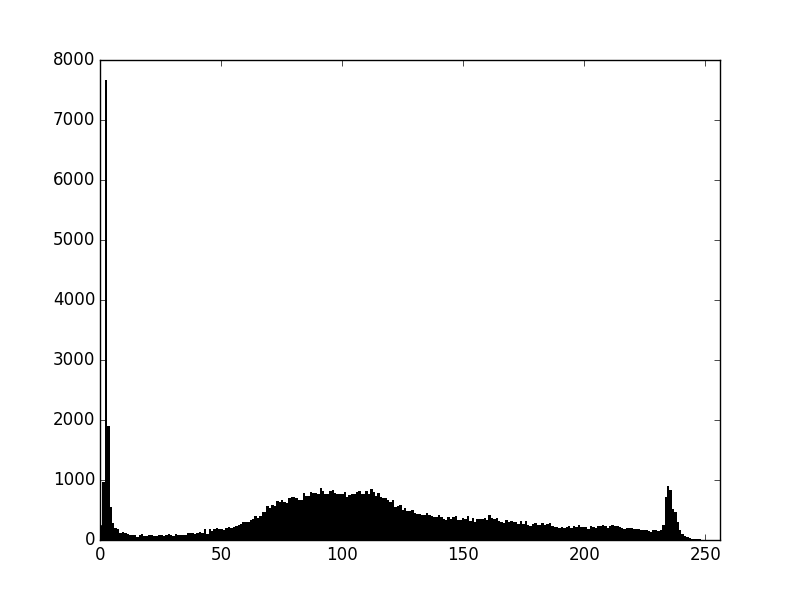
\includegraphics[width=300pt]{../result/hist.png}
	\caption{Histogram of the original image}
\end{figure}

\begin{figure}[H]
	\centering
	% pt = px * 72 / DPI
	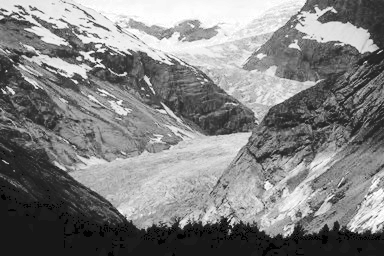
\includegraphics[width=288pt]{../result/equalize.png}
	\caption{Histogram-equalized result}
\end{figure}

\begin{figure}[H]
	\centering
	% pt = px * 72 / DPI
	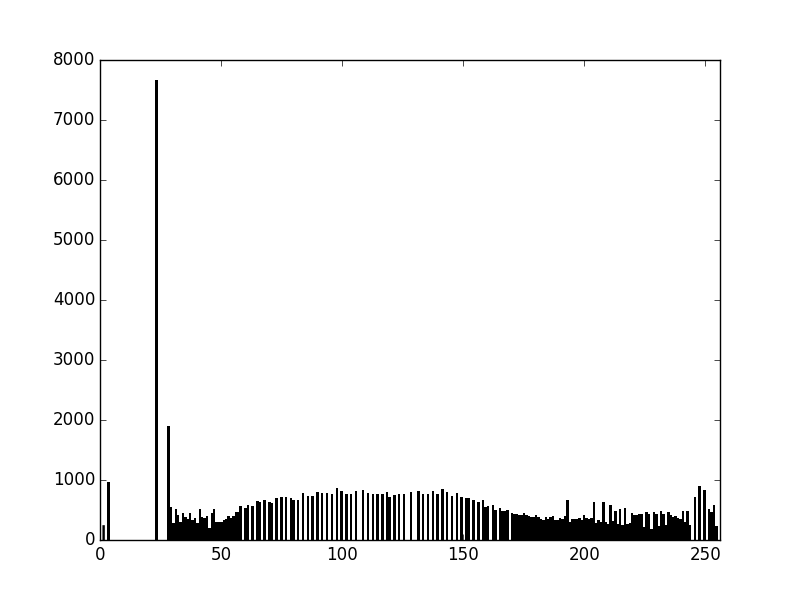
\includegraphics[width=300pt]{../result/hist-equalize.png}
	\caption{Histogram of the histogram-equalized result}
\end{figure}

% -------------------- Discussion ------------------------
\subsubsection{Discussion}

% -------------------- Algorithm ------------------------
\subsubsection{Algorithm}
\begin{algorithm}[h]
\centering
\caption{Histogram Equalization}
  \begin{algorithmic}[1]
    \Function{equalize\_hist}{$input\_img$}
      \State Create an empty image $output\_img$ with $input\_img.size$
      \If{$input\_img.level$ == $level$}
      	\State Copy $input\_img$ to $output\_img$
      	\State \Return $output\_img$
      \EndIf
      \State $new\_pallete \gets [\lfloor255 \times \frac{i}{level-1}\rfloor$ for $i$ in $[0, 1, ..., level]$]
      \For{each pixel $(x, y)$ in $input_img$}
      	\State $new\_color \gets$ the nearest neighbor of the pixel color in $new\_pallete$
      	\State Put $new\_color$ into $(x, y)$ in the $output\_img$
      \EndFor
      \State \Return $output\_img$
    \EndFunction
  \end{algorithmic}
\end{algorithm}

% -------------------- Image Patch Extraction ------------------------

\subsection{Image Patch Extraction}

% -------------------- Results ------------------------
\subsubsection{Results}
\begin{figure}[H]
	\centering
	% pt = px * 72 / DPI
	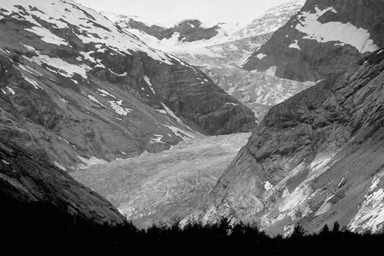
\includegraphics[width=288pt]{../img/02.png}
	\caption{The original image}
\end{figure}

\begin{figure}[H]
	\begin{minipage}[b]{0.24\linewidth}
		\centering
		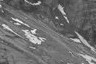
\includegraphics[width=72pt]{../result/patch-96-64-0.png}
	\end{minipage}
	\begin{minipage}[b]{0.24\linewidth}
		\centering
		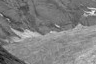
\includegraphics[width=72pt]{../result/patch-96-64-1.png}
	\end{minipage}
	\begin{minipage}[b]{0.24\linewidth}
		\centering
		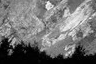
\includegraphics[width=72pt]{../result/patch-96-64-2.png}
	\end{minipage}
	\begin{minipage}[b]{0.24\linewidth}
		\centering
		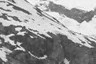
\includegraphics[width=72pt]{../result/patch-96-64-3.png}
	\end{minipage}
\end{figure}

\begin{figure}[H]
	\begin{minipage}[b]{0.24\linewidth}
		\centering
		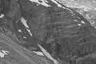
\includegraphics[width=72pt]{../result/patch-96-64-4.png}
	\end{minipage}
	\begin{minipage}[b]{0.24\linewidth}
		\centering
		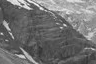
\includegraphics[width=72pt]{../result/patch-96-64-5.png}
	\end{minipage}
	\begin{minipage}[b]{0.24\linewidth}
		\centering
		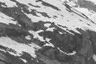
\includegraphics[width=72pt]{../result/patch-96-64-6.png}
	\end{minipage}
	\begin{minipage}[b]{0.24\linewidth}
		\centering
		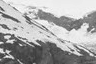
\includegraphics[width=72pt]{../result/patch-96-64-7.png}
	\end{minipage}
	\caption{96 $\times$ 64 patches}
\end{figure}

\begin{figure}[H]
	\begin{minipage}[b]{0.24\linewidth}
		\centering
		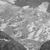
\includegraphics[width=37.5pt]{../result/patch-50-50-0.png}
	\end{minipage}
	\begin{minipage}[b]{0.24\linewidth}
		\centering
		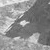
\includegraphics[width=37.5pt]{../result/patch-50-50-1.png}
	\end{minipage}
	\begin{minipage}[b]{0.24\linewidth}
		\centering
		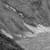
\includegraphics[width=37.5pt]{../result/patch-50-50-2.png}
	\end{minipage}
	\begin{minipage}[b]{0.24\linewidth}
		\centering
		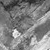
\includegraphics[width=37.5pt]{../result/patch-50-50-3.png}
	\end{minipage}
\end{figure}

\begin{figure}[H]
	\begin{minipage}[b]{0.24\linewidth}
		\centering
		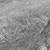
\includegraphics[width=37.5pt]{../result/patch-50-50-4.png}
	\end{minipage}
	\begin{minipage}[b]{0.24\linewidth}
		\centering
		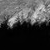
\includegraphics[width=37.5pt]{../result/patch-50-50-5.png}
	\end{minipage}
	\begin{minipage}[b]{0.24\linewidth}
		\centering
		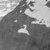
\includegraphics[width=37.5pt]{../result/patch-50-50-6.png}
	\end{minipage}
	\begin{minipage}[b]{0.24\linewidth}
		\centering
		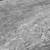
\includegraphics[width=37.5pt]{../result/patch-50-50-7.png}
	\end{minipage}
	\caption{50 $\times$ 50 patches}
\end{figure}

% -------------------- Discussion ------------------------

\subsubsection{Discussion}

% -------------------- Algorithm ------------------------
\subsubsection{Algorithm}

% -------------------- Spatial Filtering ------------------------
\subsection{Spatial Filtering}

% -------------------- Results ------------------------
\subsubsection{Results}

\begin{figure}[H]
	\centering
	% pt = px * 72 / DPI
	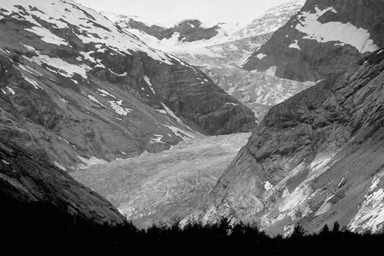
\includegraphics[width=288pt]{../img/02.png}
	\caption{The original image}
\end{figure}

\begin{figure}[H]
	\centering
	% pt = px * 72 / DPI
	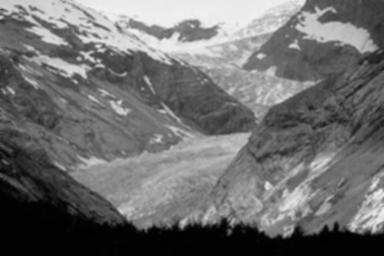
\includegraphics[width=288pt]{../result/filter-smooth-3-3.png}
	\caption{Smoothed image with $3 \times 3$ averaging filter}
\end{figure}

\begin{figure}[H]
	\centering
	% pt = px * 72 / DPI
	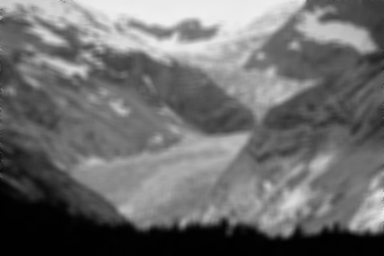
\includegraphics[width=288pt]{../result/filter-smooth-7-7.png}
	\caption{Smoothed image with $7 \times 7$ averaging filter}
\end{figure}

\begin{figure}[H]
	\centering
	% pt = px * 72 / DPI
	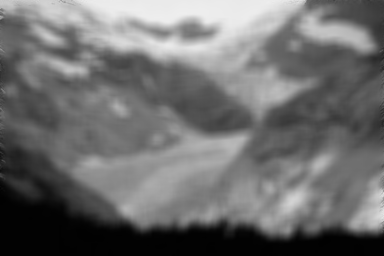
\includegraphics[width=288pt]{../result/filter-smooth-11-11.png}
	\caption{Smoothed image with $11 \times 11$ averaging filter}
\end{figure}

\begin{figure}[H]
	\centering
	% pt = px * 72 / DPI
	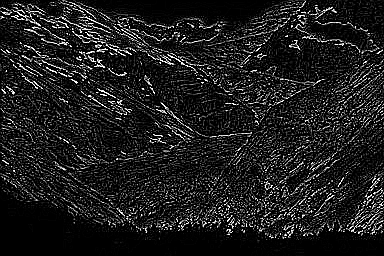
\includegraphics[width=288pt]{../result/filter-laplacian.png}
	\caption{Image filtered with $3 \times 3$ Laplacian filter}
\end{figure}

\begin{figure}[H]
	\centering
	% pt = px * 72 / DPI
	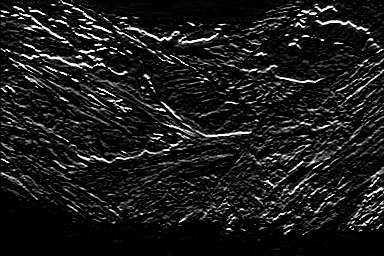
\includegraphics[width=288pt]{../result/filter-sobel-0.png}
	\caption{Image filtered with $3 \times 3$ Sobel filter}
\end{figure}

\begin{figure}[H]
	\centering
	% pt = px * 72 / DPI
	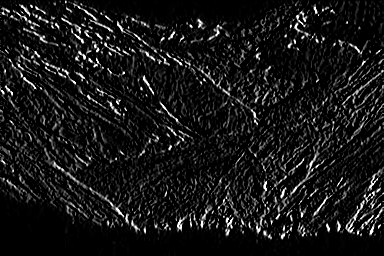
\includegraphics[width=288pt]{../result/filter-sobel-1.png}
	\caption{Image filtered with $3 \times 3$ Sobel filter}
\end{figure}

% ---------------------- Discussion ---------------------------
\subsubsection{Discussion}

% ---------------------- Algorithm ---------------------------
\subsubsection{Algorithm}
\begin{figure}[H]
	\centering
		\[ \begin{bmatrix}
			-1 & -1 & -1 \\
			-1 &  8 & -1 \\
			-1 & -1 & -1
		\end{bmatrix} \]
\caption{Laplacian filter}
\end{figure}

\begin{figure}[H]
	\centering
	\begin{minipage}[b]{0.20\linewidth}
		\[ \begin{bmatrix}
			-1 & -2 & -1 \\
			 0 &  0 &  0 \\
			 1 &  2 &  1
		\end{bmatrix} \]
		\end{minipage}
	\begin{minipage}[b]{0.20\linewidth}
		\[ \begin{bmatrix}
			-1 &  0 &  1 \\
		    -2 &  0 &  2 \\
			-1 &  0 &  1
		\end{bmatrix} \]
	\end{minipage}
	\caption{Sobel filters}
\end{figure}

\bibliographystyle{acm}

\end{document}